\chapter{Implementaciones}

\begin{comment}
Aca describo el kernel y aspectos relevantes de las versiones implementadas:
-que variables tengo que tener en cuenta en las implementaciones(por ej. el tamaño de la tabla,el rango, etc)
-que resultados espero!
-como afecta la periodicidad. la describo aca o en la parte de resultados??
-como afecta el tamaño de los bloques
\end{comment}

En este capítulo se describen los kernels implementados, incluyendo las variantes evaluadas. Además, se detalla cómo se tuvieron en cuenta los aspectos de performance expuestos en el capítulo 2.

Si bien las modificaciones están centradas puntualmente en la etapa de cálculo de las fuerzas individuales, y la evaluación sobre la performance se realizará teniendo en cuenta este paso, 
se describen aspectos de implementación de todo el método ya que son relevantes para evaluar luego la correctitud numérica de las variables químicas, la cual depdende de la iteración global del método.
Se describen, entonces, algunas optimizaciones que , si bien no son , formaron parte de la investigación realizada para este trabajo.


\section{Consideraciones previas}

Una de las primeras decisiones que se deben considerar es la precisión que se utilizará para realizar los cálculos y acumular resultados. Dadas las caracterísiticas de la arquitectura GPU, esta decisión afectará la eficiencia de cualquier cálculo a realizar y por lo tanto es uno de los factores mas importantes a analizar.

Si bien es un factor importante, este ya ha sido estudiado usando otras implementaciones del método.  En particular, se ha estudiado usando Amber\cite{le2013spfp}. El trabajo mencionado analiza un esquema mixto que implica almacenar los calculos de fuerzas entre particulas utilizando precisión simple y acumular en variables de precisión doble la suma de todos los aportes que componen la fuerza sobre una partícula. Asumiendo los resultados en performance y correctitud encontrados en Amber y,
dado que es el software con el cual evaluaremos luego la calidad numérica lograda, utilizaremos, entonces, un esquema similar de precisión para nuestra implementación.


\section{Esquema general de la implementación sobre GPU}
El esquema general utilizado para implementar el algoritmo sobre GPU es el explicado en \cite{friedrichs2009accelerating}, siguiendo el esquema explicado en detalle en el capítulo previo. 
Sin embargo, en el trabajo mencionado, el potencial incluye componentes de interacción de unión entre partículas, por lo que los calculos requeridos son algo distintos. 
En esta sección se explica, entonces, cuales son las variantes que utilizamos para realizar cada paso.

Para el primer paso de calculo de distancias entre partículas, la implementación es bastante directa. La granularidad usada es de 1 thread por cada par de partículas y se usaron tamaños de bloques fijos de 1024x1.
% Usando este esquema, con cualquier placa actual es posible lanzar en paralelo el calculo de todas las distancias para sistemas de hasta Xxx partículas. 
Teniendo en cuenta que el cálculo a realizar es  simple, no presenta posibilidades de divergencia es importante centrar la atención en el esquema de acceso a memoria para logar un uso óptimo de los recursos.

Las arquitecturas de placas de v\'ideo est\'an dise\~nadas en torno al poder de c\'omputo.
Las decisiones tomadas por los dise\~nadores de las GPUs se concentran alrededor de paralelismo a lo ancho, poniendo un gran \'enfasis en la cantidad de n\'ucleos.
En consecuencia, se dispone de menor cantidad de espacio f\'isico para m\'as memoria.

Esta decisi\'on implica que la amplia mayor\'ia de la memoria de la GPU se encuentra localizada afuera del chip.
Por lo tanto, esconder la gran latencia que tiene al acceder a la misma es parte importante del paradigma de programaci\'on para GPGPUs.

Es cr\'itico, adem\'as, que los accesos a memoria sean a direcciones m\'ultiplos de $16$, esto se conoce como \textit{accesos alineados}.
El t\'ermino \emph{coalescencia de memoria} se define en GPU como la organizaci\'on de los accesos a memoria de manera secuencial, ordenada y predecible.
Cuando la GPU accede a memoria de manera alineada, puede traer $16$, $32$ o $64$ elementos de 32 bits en una sola lectura~\cite{cudaProgrammingGuide}, suficiente para cada uno de los \threads{} del warp.
Si, en cambio, no se respeta la alineaci\'on de la memoria o los \threads{} tienen un patr\'on de pedidos impredecible, entonces se deber\'an serializar los accesos y separar en m\'ultiples transacciones a memoria global para satisfacerlos.
Este problema se agrava si se deben hacer accesos frecuentes por cientos de \threads{}, como es el caso de los bloques con gran nivel de paralelismo expl\'icito.
% Esta propiedad es muy importante para la implementación del método de dinámica molecular, ya que 
Un análisis de esto se muestra en el próximo capítulo, cuando se evalúan los efectos del tamaño de bloque.


El paso correspondiente al calculo de las fuerzas entre particulas es quizas el mas complicado de implementar, y el número de implementaciones existentes en la literatura es muy diversa, 
principalmente debido a que los calculos a realizar dependen de las interacciones que se estan utilizando y estás dan lugar a una gran variedad de posibles optimizaciones \cite{friedrichs2009accelerating}\cite{gotz2012routine}\cite{salomon2013routine}.


En el caso de interacciones \textit{non-bond}, como las que se analizan en nuestro trabajo, la principal optimizacion deriva de la propiedad de simetría que presenta el potencial de interaccion.
Es decir, la interacción entre una partícula a y b tiene el mismo modulo pero signo opuesto que el valor entre b y a. 
Esto tiene una implicación relevante en el calculo que debe realizarse ya que solo deberán calcularse interacciones para la mitad de las combinaciones entre partículas, reduciendo así considerablemente el número de cálculos.

Para hacer uso de la propiedad de simetria, entonces, el calculo de la fuerza resultante de la interaccion solo se realiza sobre $\frac{N^2}{2}$ pares, y el resto se deriva negando este valor.

% Para descomponer las componentes el cálculo se realiza usando un thread por cada par de partículas.

Para hacer la suma de la fuerza resultante, se utiliza un esquema de reduccion \cite{cudaReductions}:
Los threads ponen su contribucion al computo realizado en su posicion correspondiente de la memoria compartida, evitando tener que realizar operaciones de sincronización entre ellos. Los valores parciales se reducen,
luego, con un algoritmo paralelo en arbol: cada thread suma el valor de la posición x con el valor en 2x si este existiera. Esto se repite por la mitad de los threads, hasta que todos los valores hayan sido sumados 
y el thread 0 del bloque escribe el resultado a la memoria global.
Un esquema simplificado de esto puede verse en la figura \ref{reduction}
\begin{figure}[htbp]
   \centering
   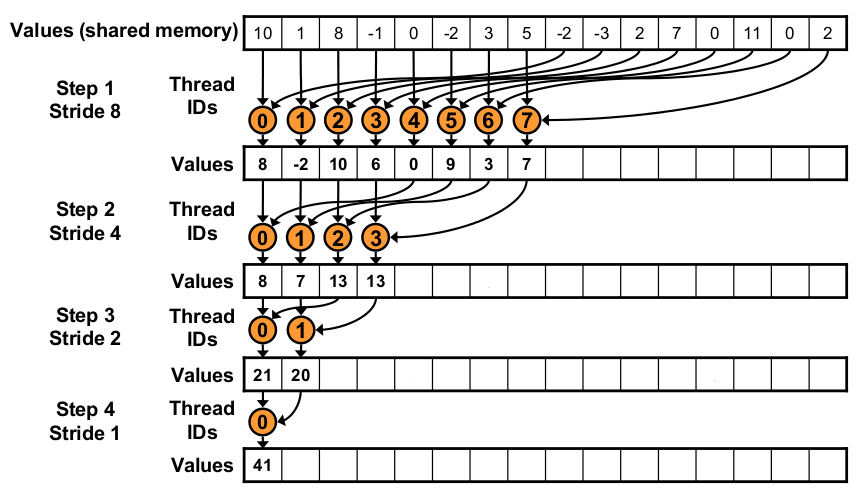
\includegraphics[width=\plotwidth]{img/md/reductions.png}
   \caption{}
   \label{reduction}
\end{figure}

Esta tecnica de reduccion es sumamente conocida para arquitecturas distribuidas, generando la respuesta en O(log 2 n) pasos. La literatura de CUDA sugiere tecnicas adicionales para minimizar aun mas el tiempo empleado en esta reducción. 
Sin embargo, al realizarse a lo sumo seis operaciones, no es necesario aplicarlas en nuestro caso particular.


Los pasos siguientes son bastante directos. La aceleración se calcula en base a la fuerza resultante usando un thread por cada partícula.
La actualización de coordenadas también se realiza usando un thread para cada partícula. El esquema de threads utilizado asegura acceso coalescente a las matrices de datos asociadas al sistema.

Para el caso de condiciones periódicas, sin embargo, hay un paso extra que se debe considerar


\section{Implementación usando tabla de potenciales}
% \subsubsection{Tabla sobre memoria global}
% \subsubsection{Tabla sobre memoria de textura}

Esta implementación solo modifica la forma en que se calcula la derivada del potencial, la cual se ejecuta ahora sobre la CPU, por lo tanto los datos de distancia y potenciales deben estar accesibles en memoria para que este cálculo pueda ser realizado.

Se implementaron variantes equivalentes para el calculo usando la ecuación derivada, usando una tabla de valores potenciales, y usando una tabla de valores de derivada.
Deberán tenerse en cuenta a la hora de usar esta implementación todos los aspectos asociados a la transferencia de datos entre la memoria del dispositivo y la memoria del host. En el próximo capitulo se verá como esta implementación es utilizada para demostrar las ventajas q aporta la arquitectura GPU.


% ****ACA PONGO LAS CARACTERISTICAS QUE OFRECE LA GPU Y QUE PUEDEN SER USADAS APROVECHANDO QUE HOY EN DIA LA MAYORIA DEL SOFT. ESTA IMPLEMENTADO SOBRE GPU*****
Para implementar este mecanismo hay varias propiedades del sistema de memoria que se puede usar y que se deben analizar......................................................
la memoria de textura provee el ajuste automatico en los limites de la tabla. Además, permite obtener el valor resultante de la interpolacion, lo cual si bien no es necesario, ayuda considerablemente en la precision.



\begin{figure}[htbp]
    \begin{lstlisting}
__global__ void potentialsMode_texture_kernel
  (double* dEr,
  double* r, 
  double cut, 
  int* item_to_type, 
  int num_samples_r, 
  int num_types, 
  int width, 
  int height)
  {
    /* Elemento de la matriz a calcular */
    /** particula 2 **/
    unsigned int x = blockIdx.x * blockDim.x + threadIdx.x;	
    /** particula 1 **/
    unsigned int y = blockIdx.y * blockDim.y + threadIdx.y;
    
    float rvalue= r[y*width+x]; 
    float result;
    
    /* Asegurarse que el thread esta dentro de los valores a calcular */
    if(x >= width || y >= height) {return;}
    if(x == y || rvalue  >= cut) 
      {
	result=0;  //fuera del cutoff
      }
      else{
      //indice 1 matriz de tipos de interacciones
      float t_o_p_1 = (float) item_to_type[y] * num_types;	
      
      //indice 2 de la matriz de tipos de interacciones
      float t_o_p_2 = (float) item_to_type[x] + 0.5 + t_o_p_1;	
      
      // convertir r en indice
      float index_x = ((rvalue - MIn) * (num_samples_r / DIST + 0.5);	
      
      //fetch valores de potencial
      float E_r_up = tex2D( texRef, index_x + DIF_FINITAS_DELTA, t_o_p_2 );
      float E_r_dwn = tex2D( texRef, index_x - DIF_FINITAS_DELTA, t_o_p_2 );
      float r_dif = DIST * 2 * (DIF_FINITAS_DELTA) / num_samples_r;
      
      //DERIVADA DISCRETIZADA
      result = (E_r_up - E_r_dwn) / (r_dif); 
      }
   
    //ESCRIBIR RESULTADOS
    dEr[y*width+x]= result;
}
    \end{lstlisting}
    \caption{Kernel utilizado para el cálculo de fuerzas a partir de una tabla de potenciales en textura}
    \label{code:potentialsKernel}
\end{figure}



\section{Implementación usando tabla de derivadas}
% \subsubsection{Tabla sobre memoria global}
% \subsubsection{Tabla sobre memoria de textura}


\begin{figure}[htbp]
    \begin{lstlisting}
__global__ void direct_derivativeMode_E_r (
    double* dEr,
    double* r, 
    double cut, 
    int* item_to_type, 
    int num_samples_r, 
    int num_types, 
    int width, 
    int height )
{ 
  /* Elemento de la matriz a calcular */
   /** particula 2 **/
  unsigned int x = blockIdx.x * blockDim.x + threadIdx.x;
  
  /** particula 1 **/
  unsigned int y = blockIdx.y * blockDim.y + threadIdx.y;	
  float rvalue= r[y*width+x]; 
  float result;
  
  /* Asegurarse que el thread esta dentro de los valores a calcular */
  if(x >= width || y >= height) {return;}
  if(x == y || rvalue  >= cut) 
    {
      result=0;  //fuera del cutoff
    }
    else{
      //indice 1 matriz de tipos de interacciones
      float t_o_p_1 = (float) item_to_type[y] * num_types;	
      
      //indice 2 matriz de tipos de interacciones
      float t_o_p_2 = (float) item_to_type[x] + 0.5 + t_o_p_1;	
      
      // convertir r en indice
      float index_x = (float)( (rvalue - MIn) * num_samples_r / DIST + 0.5);	
     
      //fetch result
      result = (double) tex2D( texRef, index_x, t_o_p_2 );
    }
   
  //ESCRIBIR RESULTADO 
  dEr[y*width+x]= result;

}
    \end{lstlisting}
    \caption{Kernel utilizado para el cálculo de fuerzas a partir de una tabla de derivadas en textura}
    \label{code:potentialsKernel}
\end{figure}



\section{Implementacion sobre CPU}

Con el fin de poder hacer una comparación real de los aspectos asociados a la performance se desarrolló además una implementación que realiza el cálculo de fuerzas sobre CPU.

